\chapter{Scenario and Problem Statement}

We consider $N$ independent, linear time-invariant (LTI) control systems sharing
a wireless communication network. Each individual sub-system $i$ consists of a
plant $\plant$, a sensor $\sensor$, and a controller $\controller$ with an
estimator $\estimator$. Every sensor $\sensor$ measures the output of the plant
periodically and sends the latest sample to $\controller$. On the controller
side, $\estimator$ estimates the current plant state based on the latest
received information. Estimated state is then used by $\controller$ to calculate
the next control input. Each controller-plant pair is assumed to be co-located,
while the sensor is operating remotely over the shared wireless channel as
illustrated in Fig.~(\ref{fig:scenario}).

\begin{figure}[htb]
  \centering
  \resizebox*{.8\columnwidth}{!}{\begin{tikzpicture}[>=latex, scale=0.9]
  \node (plant) at (0.4,6.4) [draw,minimum width=2cm,minimum height=1.5cm, rounded corners=0.1cm, text width=3cm, align=center, fill=mylightestgray] {};
  
  \node (plant) at (0.2,6.2) [draw,minimum width=2cm,minimum height=1.5cm, rounded corners=0.1cm, text width=3cm, align=center, fill=mylightergray] {};
  
  % Plant
  \node (plant) at (0,6) [draw,minimum width=2cm,minimum height=1.5cm, rounded corners=0.1cm, text width=3cm, align=center, fill=mygray] {\large{Plant $\mathcal{P}_i$}};
  
  
  % Sensor 
  \node (sensor) at (12.4,6.4) [draw,minimum width=2cm,minimum height=1.5cm, rounded corners=0.1cm, text width=3cm, align=center, fill=mylightestgray] {};
  
  \node (sensor) at (12.2,6.2) [draw,minimum width=2cm,minimum height=1.5cm, rounded corners=0.1cm, text width=3cm, align=center, fill=mylightergray] {};
  
  \node (sensor) at (12,6) [draw,minimum width=2cm,minimum height=1.5cm, rounded corners=0.1cm, text width=3cm, align=center, fill=lightgray] {\large{Sensor $\mathcal{S}_i$}};
  
  %Estimator
  \node (estimator) at (6.4,2.4) [draw,minimum width=2cm,minimum height=1.5cm, rounded corners=0.1cm, text width=3cm, align=center, fill=mylightestgray] {\large{Estimator $\mathcal{E}_i$}};

  \node (estimator) at (6.2,2.2) [draw,minimum width=2cm,minimum height=1.5cm, rounded corners=0.1cm, text width=3cm, align=center, fill=mylightergray] {\large{Estimator $\mathcal{E}_i$}};

  \node (estimator) at (6,2) [draw,minimum width=2cm,minimum height=1.5cm, rounded corners=0.1cm, text width=3cm, align=center, fill=lightgray] {\large{Estimator $\mathcal{E}_i$}};


  % Controller
  \node (controller) at (0.4,2.4) [draw,minimum width=2cm,minimum height=1.5cm, rounded corners=0.1cm, text width=3cm, align=center, fill=mylightestgray] {};
  
  \node (controller) at (0.2,2.2) [draw,minimum width=2cm,minimum height=1.5cm, rounded corners=0.1cm, text width=3cm, align=center, fill=mylightergray] {};
  
  \node (controller) at (0,2) [draw,minimum width=2cm,minimum height=1.5cm, rounded corners=0.1cm, text width=3cm, align=center, fill=lightgray] {\large{Controller $\mathcal{C}_i$}};
  
  
  % Network Cloud
  \node[cloud, cloud puffs=11, cloud ignores aspect, minimum width=2cm, minimum height=1.5, text width=2.5cm, align=center, draw] (cloud) at (12, 2) {\large {Network \\} \small{with scheduler}};
  
  % C-to-P arrow
  \draw[arrows=-triangle 45,black, ultra thick] (controller.north) -- node[pos=0.5, left] {\large $u_i[k_i]$} (plant.south);
  
  % P-to-S arrow
  \draw[arrows=-triangle 45,black, ultra thick] (plant.east) -- node[pos=0.5, above] {\large $x_i[k_i]$} (sensor.west);
  
  % P-to-Cloud arrow
  \draw[black, dashed, ultra thick] (sensor.south) -- node[] {} (cloud.north);
  
  % Cloud-to-E arrow
  \draw[arrows=-triangle 45,black, dashed, ultra thick] (cloud.west) -- node[pos=0.5, above] {} (estimator.east);

  % E-to-C arrow
  \draw[arrows=-triangle 45,black, dashed, ultra thick] (estimator.west) -- node[pos=0.5, above] {\large $\hat{x}_i[k_i]$} (controller.east);
  
  \end{tikzpicture}
} \caption[Scheme of
  $N$ sub-systems sharing a wireless communication medium]{Considered scenario
  with $N$ heterogenous LTI networked control systems. Solid lines indicate
  ideal controller-to-plant and plant-to-sensor links. Sensor-to-controller link
  is closed over a shared wireless channel. Medium access is granted centrally
  by a scheduler. Note that $k_i$ refers to the sampling period a sub-system $i$
  is in.}
  \label{fig:scenario}
\end{figure}

\section{Network Model}
Time is divided into discrete slots which are also the smallest time unit in our
scenario. We use $t \in \mathbb{N}$ to index time slots. Sensors $\sensor$
transmit state information over a wireless medium in packets containing a single
measurement. Each packet transmission starting in a slot $t$ ends within the
same slot. Medium access is granted by a centralized entity called
\textit{scheduler}. That means, in each time slot $t$, the scheduler decides
which sub-system is allowed to transmit its latest packet. Moreover, only a
single transmission resource is allocated within a single time slot. Suppose a
scheduler decision variable $\delta_i(t) \in \left\{0,1\right\}$ that takes the
value of 1 if sub-system $i$ is scheduled for transmission in slot $t$.
Then, the following holds for all time slots:

\begin{equation}
  \sum_{i=1}^{N}{\delta_i(t) \leq 1 \quad, \forall t}
\end{equation}

We consider a bursty GE channel where the link quality between each
sensor-controller pair is time and channel state dependent. (See
Sec.~{\ref{sec:GE}}) Each link is prone to its own channel state $q(t)$ which
affects successful packet reception. A packet transmitted at $t$ is lost with
probability $p_i(t) \in \left\{p_G,p_B\right\}$ or received successfully with
probability $1-p_i(t)$. Given that $\sensor$ is scheduled, let $\gamma_i(t)=1$
indicate a successful transmission with probability $\Pr[\gamma_i[t]=1 \mid
\delta_i(t)=1] = 1-p_i(t)$ and $\gamma_i(t)=0$ a failed transmission with
probability $\Pr[\gamma_i(t)=0 \mid \delta_i(t)=1] = p_i(t)$, respectively. 

% For the sake of completeness, note that $\Pr[\gamma_i[t]=1 \mid \delta_i[t]=0]
% = 0$ and $\Pr[\gamma_i[t]=0 \mid \delta_i[t]=0] = 1$. 

The control-aware scheduler is assumed to be able of measuring the instantaneous
link quality for each sub-system, thus is aware of the loss probabilities
$p_i(t)$. Further, the scheduler will make decisions by considering control and
network behaviors. The network state is comprised of variables defined in the
following.

\subsection*{Network state}

Packets are generated periodically at $\sensor$ every $D_i \in \mathbb{Z}^+$
slots. We call the generation of a packet a \textit{sampling event} and the time
between two consecutive sampling events a \textit{sampling period}. Let $t_{i,o}
\sim \mathcal{U}[0, D_i)$ denote the initial sampling event of sub-system $i$,
then the set of slots in which a sampling event occurs are:

\begin{equation}
  \mathcal{G}_i \triangleq \lbrace t_{i,o}, \; t_{i,o} + D_{i}, \; t_{i,o} + 2 D_{i}, \; \dots \rbrace 
\end{equation}

As $t_{i,o}$ is an uniformly distributed random variable and not necessarily
equal for each sub-system, we allow sampling to operate in a non-synchronized
fashion. 

Having received an update, the controller does not benefit from receiving an
older plant measurement \cite{costa2016age}. Older packets are considered to be
``non-informative'' and obsolete. Therefore, sensors replace their packet in the
transmit buffer with a more recent measurement upon arrival of a new update. We
define a variable $t_{i,g}(t)$ that denotes the generation time of the packet
waiting for transmission at $\sensor$. As packets are solely generated during a
sampling event, $t \in \mathcal{G}_i$ are the only slots, in which $t_{i,g}$ is
updated. Thus, $t_{i,g}$ evolves as follows:

\begin{equation}
  t_{i,g}(t+1) =
  \begin{cases}
  t+1 & \text{, if } t+1 \in \mathcal{G}_i \\
  t_{i,g}(t) & \text{, otherwise}	
  \end{cases}
\end{equation}

We further define $t_{i,r}(t)$ as the generation time of the newest packet
received by $\controller$ until time $t$:

\begin{equation}
  t_{i, r}(t+1) =
  \begin{cases}
  t_{i, g}(t) & \text{, if } \delta_i(t) \cdot \gamma_i(t) = 1 \\
  t_{i, r}(t) & \text{, otherwise}	
  \end{cases}
\end{equation}

Fig.~(\ref{fig:ageplot}) shows an exemplary evolution of $t_{i,g}$, along with
the relationship between ${t_{i,r}(t+1)}$ and $t_{i,g}(t)$ after two successful
updates. Generation time $t_{i,g}$ demonstrates a discrete staircase behavior at
$t \in \mathcal{G}_i$, while received time $t_{i,r}$ can take new values at any
slot $t \in \mathbb{N}$ subject to the indication variables $\delta_i$ and
$\gamma_i$.

\begin{figure}[htb]
  \centering
  \resizebox*{.6\columnwidth}{!}{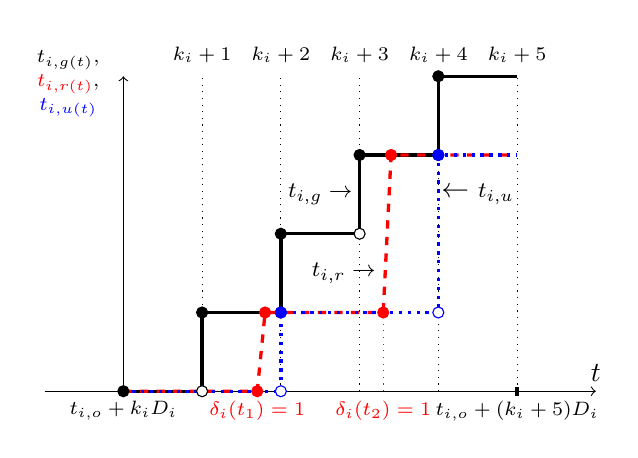
\begin{tikzpicture}

% horizontal axis
\draw[->] (-1,0) -- (6,0) node[anchor=south] {$t$};
% labels
\draw	(0,4.5) node[anchor=east] {}
		(1,4.5) node[anchor=north] {\scriptsize$k_i+1$}
		(2,4.5) node[anchor=north] {\scriptsize$k_i+2$}
		(3,4.5) node[anchor=north] {\scriptsize$k_i+3$}
		(4,4.5) node[anchor=north] {\scriptsize$k_i+4$}
		(5,4.5) node[anchor=north] {\scriptsize$k_i+5$}
		(0,-0.0) node[anchor=north]
		{\scriptsize$t_{i,o} + k_i D_i$}
		(5,-0.0) node[anchor=north]
		{\scriptsize$t_{i,o}+(k_i+5)D_i$}
		(1.7,-0.0) node[anchor=north] {\color{red}\scriptsize$\delta_i(t_1)=1$}
		(3.3,-0.0) node[anchor=north] {\color{red}\scriptsize$\delta_i(t_2)=1$};

\node[] at (-0.7, 4.2) {\scriptsize$t_{i,g(t)}$,};
\node[] at (-0.7, 3.9) {\color{red}{\scriptsize$t_{i,r(t)}$}\color{black}{\scriptsize,}};
\node[] at (-0.7, 3.6) {\color{blue}{\scriptsize$t_{i,u(t)}$}};

\draw[very thick, black] (5,-0.06) --  (5,+0.06);
	
% vertical axis
\draw[->] (0,0) -- (0,4) node[anchor=east] {};
% vertical ticks
\draw[dotted] (1,0) -- (1,4);
\draw[dotted] (2,0) -- (2,4);
\draw[dotted] (3,0) -- (3,4);
\draw[dotted] (4,0) -- (4,4);
\draw[dotted] (5,0) -- (5,4);
\draw[dotted,red] (3.3,0) -- (3.3,1);

% Delta 1
%\draw[very thick, black, solid] (0,1) -- (1,1);
%\draw[very thick, black, solid] (1,0) -- (2,0);
%\draw[very thick, black, solid] (2,1) -- (3,1);
%\draw[very thick, black, solid] (3,2) -- (4,2);
%\draw[very thick, black, solid] (0,1) -- (1,1);
%\draw[very thick, black, solid] (0,1) -- (1,1);
\draw[very thick, black, solid] (0,0) --  (1,0) -- (1,1) -- (2,1) -- (2,2) -- (3,2) --  (3,3) -- (4,3) -- (4,4)-- (5,4);

\draw[very thick, red, dashed] (0,0) --  (1.7,0) -- (1.8,1) -- (3.3,1) -- (3.4,3) -- (5,3);

\draw[very thick, blue, dotted] (0,0) --  (2,0) -- (2,1) -- (4,1) -- (4,3) -- (5,3);

%\draw (-.7, 1) node {\scriptsize$\Delta[k-1]$}; %label
\draw (2.5, 2.5) node { \footnotesize$t_{i,g}\rightarrow$};

\draw (2.8, 1.5) node { \footnotesize$t_{i,r}\rightarrow$};

\draw (4.5, 2.5) node { $\leftarrow\,\,$\footnotesize$t_{i,u}$};



\node[circle,draw=black, fill=white, inner sep=0pt,minimum size=4pt] (b) at (1,0) {};
\node[circle,draw=black, fill=white, inner sep=0pt,minimum size=4pt] (b) at (2,1) {};
\node[circle,draw=black, fill=white, inner sep=0pt,minimum size=4pt] (b) at (3,2) {};
\node[circle,draw=black, fill=white, inner sep=0pt,minimum size=4pt] (b) at (4,3) {};


\node[circle,draw=black, fill=black, inner sep=0pt,minimum size=4pt] (b) at (0,0) {};
\node[circle,draw=black, fill=black, inner sep=0pt,minimum size=4pt] (b) at (1,1) {};
\node[circle,draw=black, fill=black, inner sep=0pt,minimum size=4pt] (b) at (2,2) {};
\node[circle,draw=black, fill=black, inner sep=0pt,minimum size=4pt] (b) at (3,3) {};
\node[circle,draw=black, fill=black, inner sep=0pt,minimum size=4pt] (b) at (4,4) {};
%\node[circle,draw=black, fill=black, inner sep=0pt,minimum size=4pt] (b) at (5,4) {};

\node[circle,draw=blue, fill=white, inner sep=0pt,minimum size=4pt] (b) at (2,0) {};
\node[circle,draw=blue, fill=white, inner sep=0pt,minimum size=4pt] (b) at (4,1) {};



\node[circle,draw=blue, fill=blue, inner sep=0pt,minimum size=4pt] (b) at (2,1) {};
\node[circle,draw=blue, fill=blue, inner sep=0pt,minimum size=4pt] (b) at (4,3) {};


\node[circle,draw=red, fill=red, inner sep=0pt,minimum size=4pt] (b) at (1.7,0) {};
\node[circle,draw=red, fill=red, inner sep=0pt,minimum size=4pt] (b) at (3.3,1) {};



\node[circle,draw=red, fill=red, inner sep=0pt,minimum size=4pt] (b) at (1.8,1) {};
\node[circle,draw=red, fill=red, inner sep=0pt,minimum size=4pt] (b) at (3.4,3) {};


\end{tikzpicture}
} 
  \caption[Example evolution of generation time $t_{i,g}$, received time
  $t_{i,r}$ and update time $t_{i,g}$]{Evolution of generation time
  $t_{i,g}(t)$, received time $t_{i,r}(t)$ and the update time $t_{i,g}(t)$
  depicted in y-axis versus time in x-axis. $t_{i,g}(t)$ and $t_{i,u}(t)$ are
  updated periodically with $D_i$ slots, while $t_{i,r}(t)$ can be updated
  asynchronously. On x-axis with $\delta_i(t_{1,2})=1$ two cases of successful
  packet transmission for sub-system $i$ are depicted.}
  \label{fig:ageplot}
\end{figure}  

\section{Control Model}

The system of the $i$-th plant $\plant$ is considered to evolve by the following
LTI model over discrete time:

\begin{equation}
  \label{eq:discretemodel}
  \boldsymbol{x}_i[k_i+1] = \boldsymbol{A}_i \boldsymbol{x}_i[k_i] + \boldsymbol{B}_i \boldsymbol{u}_i[k_i] + \boldsymbol{w}_i[k_i]
\end{equation}

with time-invariant system matrix $\boldsymbol{A}_i \in \mathbb{R}^{n_i\times
n_i}$ and input matrix $\boldsymbol{B}_i \in \mathbb{R}^{n_i\times m_i}$. System
noise is denoted by $\boldsymbol{w}_i \in \mathbb{R}^{n_i}$ which is
characterized by a multi-variate Gaussian distribution with zero mean and
diagonal covariance matrix $\mathbf{\Sigma}_i \in \mathbb{R}^{n_i}$, i.e.,
$\boldsymbol{w}_i \sim \mathcal{N}(\mathbf{0}, \mathbf{\Sigma}_i)$. We assume
the sub-systems to operate slower than the network. In other words, the plant
state changes only after each sampling event and remains constant until the next
one. Thus, the discrete dynamics of sub-systems as described in
Eq.~\eqref{eq:discretemodel} is indexed by a different time variable $k_i$. It
indicates in which sampling period a sub-system currently is and can be obtained
at any time slot $t$ with:

\begin{equation}
  \label{eq:k_map}
	k_i(t) = \floor{\frac{t - t_{i,o}}{D_i}}
\end{equation}

In addition, $\boldsymbol{x}_i[k_i] \in \mathbb{R}^{n_i}$ and
$\boldsymbol{u}_i[k_i] \in \mathbb{R}^{m_i}$ represent the system state and
control input in sampling period $k_i$, respectively. At the beginning of each
sampling period $k_i$, i.e., at $t=t_{i,o}+k_iD_i$, the controller $\controller$
calculates $\boldsymbol{u}_i[k]$ given the available observation history. The
obtained control input is then applied to $\plant$ during the same sampling
period. As a result, any packet arriving in sampling period $k_i$ after
$\boldsymbol{u}_i[k_i]$ is calculated, will be queued until it is first utilized
in the next control input $\boldsymbol{u}_i[k_i+1]$. To capture the
aforementioned update delay of successfully received packets, we introduce
$t_{i,u}(t)$ as the generation time of the latest utilized packet by
$\controller$:

\begin{equation}
  \label{eq:t_u}
  t_{i, u}(t+1) =
  \begin{cases}
  t_{i, r}(t+1) & \text{, if } t+1 \in \mathcal{G}_i \\ 
  t_{i, u}(t) & \text{, otherwise}	
  \end{cases} 
\end{equation}

Time dynamics of $t_{i,u}$ is seen in Fig.~(\ref{fig:ageplot}) where it takes
the value of $t_{i,r}$ at the end of a control system period $t \in
\mathcal{G}_i$.

\subsection*{Age-of-Information Model}
The discrete-time model allows for communication and control to evolve in
different time steps. Particularly, in control, changes occur at sampling
events. Thus, in a control application's point of view, plant observations
included in packets age only every $D_i$ slots. Information staleness is then
expressed in multiples of $D_i$. Therefore, we define AoI as the number of
sampling periods elapsed since the generation of the freshest information at
$\controller$ and can be determined at any slot $t$ as:

\begin{equation}
  \label{eq:aoi}
  \Delta_i(t) = \ceil{\dfrac{t - t_{i,u}(t)}{D_{i}}} 
\end{equation}

It is important to understand that, since packets arrive at least one slot
delayed, they can never be utilized to compute the control input of the same
sampling period in which they are received. Hence, the minimum AoI in our
scenario is one, i.e., $\Delta_i(t) \ge 1,\forall i,t$.

\subsection*{Remote Estimation and Control Law}
In order to compensate for network-induced packet loss and limited network
resources, we consider an \textit{estimation-based controller}. Each controller
$\controller$ employs a Kalman-like state estimator $\estimator$ based on the
assumptions that both are aware of the control system parameters
$\boldsymbol{A}_i, \boldsymbol{B}_i, \boldsymbol{w}_i$ as well as $t_{i,o}$ and
$D_i$. These are motivated by the time-invariant nature of the sub-system's
dynamics and enabling the estimation-based controller to map any $t$ to $k_i$ by
using Eq.~\eqref{eq:k_map}. In turn, the controller can determine the AoI of its
most up-to-date plant state information $\boldsymbol{x_i}[k_i-\Delta_i[k_i]]$
that is $\Delta_i[k_i]$ sampling periods old.

Combining our assumptions, each estimator $\estimator$ predicts the current
plant state as a conditional expectation, i.e., $\hat{\boldsymbol{x}}_i[k_i] =
\E\left[\boldsymbol{x}_i[k_i] \mid \Delta_i[k_i],\boldsymbol{x}_i[k_i-\Delta_i]
\right]$. We leverage the results in \cite{ayan2019age}, that the minimal mean
squared estimation error is achieved by:

\begin{equation}
  \label{eq:estimatedstate}
    \boldsymbol{\hat{x}}_i[k_i] = \boldsymbol{A}_i^{\Delta_i[k_i]} \,  \boldsymbol{x}_i[k_i - \Delta_i[k_i]] + \sum_{q=1}^{\Delta_i[k_i]} \boldsymbol{A}_i^{q - 1} \, \boldsymbol{B}_i \, \boldsymbol{u}_i [k_i - q].
\end{equation}

To perform this estimation, $\estimator$ has to keep track of the last
$\Delta_i[k_i]$ control inputs. However, this does not involve any additional
communication effort since this information is generated locally and thus
already present at $\estimator$.

Further, with Eq.~\eqref{eq:discretemodel} and \eqref{eq:estimatedstate} the
estimation error $\boldsymbol{e}_i[k_i]$ is obtained as:

\begin{equation}
  \boldsymbol{e}_i[k_i] \triangleq \boldsymbol{x}_i[k_i] - \boldsymbol{\hat{x}}_i[k_i] = \sum_{q=1}^{\Delta_i[k_i]} \boldsymbol{A}_i^{q-1} \, \boldsymbol{w}_i[k_i - q].
\end{equation}

By taking the mean-squared norm of $\boldsymbol{e}_i[k_i]$ the expected mean
squared error (MSE) at $\controller$ is expressed by:

\begin{align}
  \label{eq:estimationerror}
  \E \left[ \left(\boldsymbol{e}_i[k_i]\right)^T \, \boldsymbol{e}_i[k_i]\right] & = \sum_{r=1}^{\Delta_i[k_i] - 1} \tr \left( \left(\boldsymbol{A}_i^T\right)^r  \left(\boldsymbol{A}_i \right)^r \boldsymbol{\Sigma}_i \right) \\ \nonumber
  & \triangleq g(\Delta_i[k_i]).
\end{align}

The derivations are found in \cite{ayan2019age}. It is important to note that
Eq.~\eqref{eq:estimationerror} is only a function of AoI $\Delta_i[k_i]$ and
independent from the actual system state $\boldsymbol{x}_i[k_i]$. This would not
be true in the case of time-invariant control systems. Here, we define the
$g(\Delta_i[k_i])$ as an age-penalty function that penalizes high estimation
errors and will be subject to minimization in the scheduling problem. 

After obtaining a state estimation, it is utilized in calculating the control
input according to the control law:

\begin{equation}
  \label{eq:controllaw}
  \boldsymbol{u}_i[k_i] = - \boldsymbol{L}_i^* \,\boldsymbol{\hat{x}}_i[k_i],
\end{equation}

where $\boldsymbol{L}_i^* \in \mathbb{R}^{m_i \times n_i}$ is the optimal state
feedback gain matrix. $\boldsymbol{L}^*_i$ is obtained from:

\begin{equation}
  \label{eq:optimalgain}
  \boldsymbol{L}_i^* = \left(\boldsymbol{R}_i + \boldsymbol{B}_i^T \boldsymbol{P}_i \boldsymbol{B}_i \right)^{-1} \boldsymbol{B}_i^T \boldsymbol{P}_i \boldsymbol{A}_i,
\end{equation}

which solves the discrete time algebraic Riccati equation:
\begin{equation}
  \label{eq:riccati}
  \boldsymbol{P}_i = \boldsymbol{Q}_{i} + \boldsymbol{A}_i^T \left(\boldsymbol{P}_i - \boldsymbol{P}_i \boldsymbol{B}_i ( \boldsymbol{R}_{i} + \boldsymbol{B}_i^T \boldsymbol{P}_i \boldsymbol{B}_i)^{- 1} \boldsymbol{B}_i^T \boldsymbol{P}_i \right) \boldsymbol{A}_i.
\end{equation}

$\boldsymbol{Q}_{i}$ and $\boldsymbol{R}_{i}$ are weighting matrices of
appropriate size that penalize the state and control inputs in the infinite
horizon, \textit{linear-quadratic-Gaussian} (LQG) cost function $F_i$:

\begin{equation}
  F_i = \dfrac{1}{K} \limsup_{K \rightarrow \infty} \sum_{k_i=0}^{K-1} (\boldsymbol{x}_i[k_i])^T \boldsymbol{Q}_i \boldsymbol{x}_i[k_i] +  (\boldsymbol{u}_i[k_i])^T \boldsymbol{R}_i \boldsymbol{u}_i[k_i]. 
\end{equation}

One can interpret $F_i$ as an indicator of control performance. The lower $F_i$
is, the higher is the \textit{quality of control} QoC.

\section{Scheduling Problem Formulation} \label{sec:problem}

From Eq.~\eqref{eq:estimationerror} it becomes evident, that expected estimation
performance is controlled by the AoI of sub-systems. By scheduling a certain
control application, information with lower $\Delta_i[k_i]$ is provided to its
estimator, resulting in low age-penalties. Accounting MSE as a cost function,
our goal is to derive a scheduler that maximizes overall estimation accuracy by
minimizing the total expected cost. 

We are interested in the class of scheduling policies $\pi$ that consists of a
sequence of scheduling decisions $\mu(t') \in \left\{\varnothing,1,\dots,N
\right\}$ for the next $H \in \mathbb{Z}^+$ slots, i.e.,
$\pi=\left\{\mu(t),\dots\mu(t+H-1) \right\}$. $H$ is the \textit{finite horizon}
parameter that defines how many future slots are being considered. Thus, $H$
controls the ``farsightedness'' of the proposed scheduler.

Let us define the network state $\boldsymbol{s} \in \mathbb{Z}^{4\cdot N}$ as:

\begin{equation}
  \boldsymbol{s}(t) \triangleq \left[\boldsymbol{t}_g(t) \quad \boldsymbol{t}_r(t) \quad \boldsymbol{t}_u(t) \quad \boldsymbol{q}(t)\right]^T, 
\end{equation} 
with: 
\begin{align}
  \boldsymbol{t}_g(t) &\triangleq \left[ t_{1,g}(t) ~ \dots ~ t_{N,g}(t) \right]^T ,\\
  \boldsymbol{t}_r(t) &\triangleq \left[ t_{1,r}(t) ~ \dots ~ t_{N,r}(t) \right]^T ,\\
  \boldsymbol{t}_u(t) &\triangleq \left[ t_{1,u}(t) ~ \dots ~ t_{N,u}(t) \right]^T ,\\
  \boldsymbol{s}(t) &\triangleq \left[ q_1(t) ~ \dots ~ q_N(t) \right].
\end{align}

Each $\mu(t)$ maps the current network to a scheduling decision which indexes
sub-system that is granted medium access $\mu(t)=i$ implies
$\delta_i(t)=1$. 
